\let\negmedspace\undefined
\let\negthickspace\undefined
\documentclass[journal]{IEEEtran}
\usepackage[a5paper, margin=10mm, onecolumn]{geometry}
\usepackage{lmodern} % Ensure lmodern is loaded for pdflatex

\setlength{\headheight}{1cm} % Set the height of the header box
\setlength{\headsep}{0mm}     % Set the distance between the header box and the top of the text

\usepackage{gvv-book}
\usepackage{gvv}
\usepackage{cite}
\usepackage{amsmath,amssymb,amsfonts,amsthm}
\usepackage{algorithmic}
\usepackage{graphicx}
\graphicspath{{./figs/}}
\usepackage{textcomp}
\usepackage{xcolor}
\usepackage{txfonts}
\usepackage{listings}
\usepackage{enumitem}
\usepackage{mathtools}
\usepackage{gensymb}
\usepackage{comment}
\usepackage[breaklinks=true]{hyperref}
\usepackage{tkz-euclide} 
\usepackage{listings}
\usepackage{gvv}                                        
\def\inputGnumericTable{}                                 
\usepackage[latin1]{inputenc}                                
\usepackage{color}                                            
\usepackage{array}                                            
\usepackage{longtable}                                       
\usepackage{calc}                                             
\usepackage{multirow}                                         
\usepackage{hhline}                                           
\usepackage{ifthen}                                           
\usepackage{lscape}
\usepackage{circuitikz}
\tikzstyle{block} = [rectangle, draw, fill=blue!20, 
text width=4em, text centered, rounded corners, minimum height=3em]
\tikzstyle{sum} = [draw, fill=blue!10, circle, minimum size=1cm, node distance=1.5cm]
\tikzstyle{input} = [coordinate]
\tikzstyle{output} = [coordinate] 



\begin{document}
	
	\bibliographystyle{IEEEtran}
	\vspace{3cm}
	
	\title{1.5.35}
	\author{EE25BTECH11048 - Revanth Siva Kumar.D}
	\maketitle
	% \newpage
	% \bigskip
	{\let\newpage\relax\maketitle}
	
	\renewcommand{\thefigure}{\theenumi}
	\renewcommand{\thetable}{\theenumi}
	\setlength{\intextsep}{10pt} % Space between text and floats
	
	
	\numberwithin{equation}{enumi}
	\numberwithin{figure}{enumi}
	\renewcommand{\thetable}{\theenumi}
	
	\textbf{Question}:The mid-point of segment $AB$ is the point $P(0,4)$. If the coordinates of $B$ are $(-2,3)$ then the coordinates of $A$ are \underline{\hspace{1.5cm}}. 

\solution\\\textbf{Given Information}  

The midpoint of segment $AB$ is $P(0,4)$.  

The coordinates of point $B$ are $(-2,3)$.  

We need to find the coordinates of point $A$ using a specific matrix method based on the section formula.  

\textbf{Matrix Setup}  

First, write the coordinates of the points as column matrices:  

\begin{align*}
    P = \myvec{0 \\ 4}, 
\end{align*}
\begin{align*}
    B = \myvec{-2 \\ 3}, 
\end{align*}
\begin{align*}
    A = \myvec{x \\ y}
\end{align*}



\textbf{The Formula}  

Since $P$ is the midpoint, it is known that $A$ divides $BP$ in the ratio -2:1 internally or in other words 2:1 externally.
Here k = -2, Thus by section formula:
\begin{align*}
A = \frac{kP+B}{1+k}
\end{align*}
Substituting k = -2 we get
\begin{align*}
    A = 2P - B
\end{align*}


\textbf{Calculation}  

Substitute the matrices:  
\begin{align*}
    A = 2 \myvec{0 \\ 4} - \myvec{-2 \\ 3}
\end{align*}



Scalar multiplication:  
\begin{align*}
    A = \myvec{0 \\ 8} - \myvec{-2 \\ 3}
\end{align*}


Matrix subtraction:  
\begin{align*}
A = \myvec{0 - (-2) \\ 8 - 3} 
= \myvec{2 \\ 5}    
\end{align*}



\textbf{Conclusion} 

The coordinates of point $A$ are $(2,5)$.  

Quick check: midpoint of $A(2,5)$ and $B(-2,3)$ is  
\begin{align*}
    \left(\frac{2+(-2)}{2}, \frac{5+3}{2}\right) = (0,4) = P
\end{align*}

 

\begin{figure}[H]
    \centering
    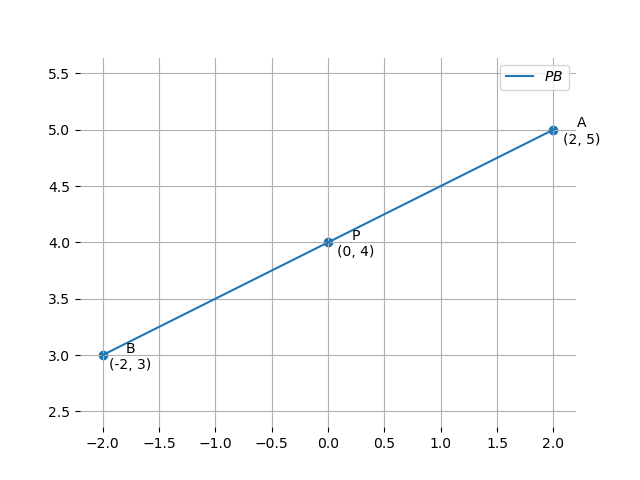
\includegraphics[width=0.5\columnwidth]{figs/Figure_1.png}
    \caption{GRAPH PLOT USING PYTHON ONLY}
    \label{fig:placeholder}
\end{figure}

\begin{figure}[H]
    \centering
    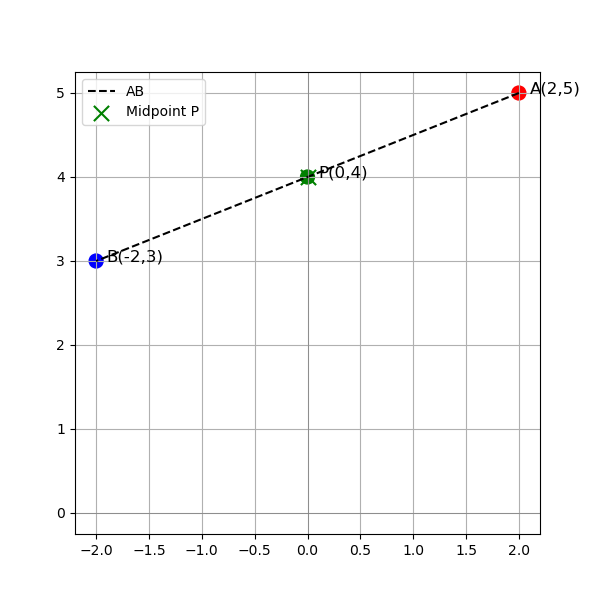
\includegraphics[width=0.5\columnwidth]{figs/Figure_2.png}
    \caption{GRAPH PLOT USING SHARED OUTPUT FROM C}
    \label{fig:placeholder}
\end{figure}
\end{document}

